% not fixed

\chapter{TINJAUAN PUSTAKA}
\label{chap:tinjauanpustaka}

% Ubah bagian-bagian berikut dengan isi dari tinjauan pustaka

\section{\textit{State of Art}}
\label{sec:penelitianterdahulu}
% state of the art

\subsection{Penelitian Berkaitan dengan \textit{Smart Whiteboard}}
\label{subsec:penelitianterkaitsmartwhiteboard}
Kellerman et al. \citep*{kellerman2018smart} mencoba untuk menyediakan suatu cara alternatif dan terjangkau pada papan tulis atau slides agar bisa mendapat interaksi lebih dari murid serta untuk meningkatkan efisiensi dari pengajaran. Pada penelitiannya, peneliti membuat sebuah papan tulis interaktif menggunakan Nintendo Wii \textit{Remote} dan \textit{PC Suite}. \textit{Software Suite} yang dikembangkan memungkinkan tampilan PC apapun dapat digunakan sebagai papan tulis interaktif. Sistem yang dibangun memiliki fungsi yang diperlukan untuk menciptakan sarana pembelajaran yang lebih baik dan lebih berteknologi, serta memberi pengguna dan siswa alat tambahan untuk menunjang Pendidikan interaktif. \textit{PC Suite} dibuat seramah mungkin sehingga dapat digunakan dengan mudah pada komputer standar. \par

\subsection{Penelitian Berkaitan dengan \textit{Word Detection}}
\label{subsec:penelitianterkaitworddetection}
Arun et al. \citep*{arun2019handwritten} menyajikan pendekatan sederhana untuk segmentasi huruf kata tulisan tangan menggunakan pendekatan bounding box dan pendekatan berbasis pixel. Segmentasi huruf tulisan tangan merupakan proses yang menantang karena gaya penulisan yang bervariasi. Kata-kata tulisan tangan yang tidak bersentuhan disegmentasikan dengan pendekatan bounding box dan kata-kata tulisan tangan yang bersentuhan disegmentasi menggunakan pendekatan pixel. Paper ini mencapai tingkat segmentasi hingga 94.45\% dan tingkat pengenalan 85.89\% dengan skema training dan testing 50-50\%. \par

\subsection{Penelitian Berkaitan dengan YOLO \textit{Object Detection}}
\label{subsec:penelitianterkaityolo}
Karlina dan Indarti \citep*{karlina2020pengenalan} membuat pengenalan objek Makanan cepat saji dari \textit{video} dan \textit{real time webcam} menggunakan metode \textit{deep learning. You Only Look Once (YOLO)} merupakan model \textit{deep learning} yang digunakan untuk pengenalan objek. Jumlah data yang digunakan terdiri dari 468 gambar yang terdiri dari 3 jenis Makanan cepat saji. Nilai avg loss pada model akhir yang dibangun yaitu 4.6\%, nilai validasi mAP 100\%, serta akurasi akhir berkisar antara 63\% sampai 100\%. \par

% Per Teori Penunjang dibuat section baru

% papan tulis
% image processing

\section{\textit{Citra}}
\label{sec:citra}

Citra atau gambar merupakan representasi visual dari suatu objek, orang, atau pemandangan. Gambar digital terdiri dari elemen gambar yang juga dikenal sebagai piksel. Gambar digital adalah fungsi 2 dimensi f(x,y) yang merupakan proyeksi pemandangan 3 dimensi kedalam bidang proyeksi 2 dimensi dimana x dan y mewakili lokasi piksel dan mengandung intensitas nilai. Adapun jika nilai x,y, dan intensitas bersifat diskrit, maka citra tersebut dapat dikatakan sebagai citra digital \citep*{tyagi2018understanding}.

\section{\textit{Image Processing}}
\label{sec:imageprocessing}
Citra direpresentasikan dalam bentuk matriks numerik yang memiliki informasi intensitas atau warna pada tiap elemen gambar. Karena itu operasi matematika sangat penting dalam berbagai proses pengolahan citra. Dalam pelaksanaan proses pengolahan citra, sebagian proses dilakukan dalam citra skala abu-abu (\textit{grayscale}). Adapun untuk pengolahan citra berwarna, mulanya citra berwarna tersebut dapat didekomposisi menjadi komponen merah, hijau, dan biru dan masing-masing komponen diproses secara independen sebagai citra \textit{grayscale} \citep*{tyagi2018understanding}. Secara umum, proses pengolahan citra terbagi menjadi 3 tingkatan sebagai berikut:
\begin{enumerate}
    \item \textit{Low-Level Image Processing. \textnormal{Pada} low-level image processing, input \textnormal{dan} output} adalah berupa gambar dan proses yang dilakukan merupakan operasi sederhana. Adapun contoh dari \textit{low-level image processing} yaitu seperti \textit{contrast enhancement \textnormal{dan} noice reduction.}  
    \item \textit{Mid-Level Image Processing. \textnormal{Pada} mid-level image processing,} proses yang dilakukan merupakan operasi yang melibatkan ekstraksi atribut dari suatu citra. Adapun contoh dari \textit{mid-level image processing \textnormal{yaitu seperti} Edges, Contours, \textnormal{dan} Regions.}
    \item \textit{High-Level Image Processing. \textnormal{Pada} high-level image processing,} proses yang dilakukan merupakan operasi kompleks yang berkaitan dengan analisis dan interpretasi konten untuk pengambilan keputusan.
\end{enumerate} 

\section{\textit{Deep Learning}}
\label{sec:deeplearning}
\textit{Deep learning} adalah serangkaian algoritma dalam \textit{machine learning} yang mempelajari fitur-fitur dari sebuah data mentah secara otomatis. \textit{Deep learning} merupakan cabang dari \textit{machine learning} yang didasarkan pada \textit{artificial neural network}. \textit{Artificial neural network} terinspirasi dari arsitektur saraf otak manusia, dan seperti halnya otak manusia, \textit{artificial neural network} terdiri dari berbagai neuron. Seperti \textit{neural network} tradisional, \textit{deep neural network} juga terdiri dari neuron buatan yang disusun dalam bentuk \textit{input layer, hidden layer, \textnormal{dan} output layer}. Namun, tidak seperti \textit{neural network} tradisional, jumlah \textit{hidden layer \textnormal{pada} deep neural network} umumnya lebih dari 1 \textit{layer} \citep*{ahmad2019deep}. 
% \textit{Deep learning} memungkinkan model komputasi dari beberapa lapisan pemrosesan untuk mempelajari dan mewakili data dengan berbagai tingkat abstraksi. 
% \textit{Deep learning} merupakan metode yang memiliki implementasi sangat banyak mencakup \textit{neural Networks, hierarchical probabilistic models, unsupervised learning} dan \textit{supervised learning} \citep*{voulodimos2018deep}. 
\textit{Deep Learning} dirancang untuk dapat terus mengolah data dan menganalisa data tersebut seperti dalam mengambil keputusan. 
Adapun dalam \textit{Deep Learning, training} suatu data dipengaruhi oleh banyaknya jumlah layer dan jumlah neuron. Artinya, semakin banyak layer atau neuron yang digunakan maka akan semakin lama proses yang dilakukan, hal ini disebabkan oleh tingkat kompleksitas yang semakin besar juga. \par

Seperti \textit{machine learning, deep learning} juga memiliki beragam pendekatan dalam mempelajari suatu dataset. Secara umum, pendekatan \textit{deep learning} dapat dikategorikan kedalam 3 kelompok yaitu: \textit{Deep network for supervised learning, Deep Network for unsupervised learning,} dan hybrid. 
Adapun pada penelitian ini menggunakan CNN yaitu pendekatan dengan \textit{deep network for supervised learning,} hal ini dapat terlihat terlihat dari input dataset yang akan dilatih telah memiliki label atau kelas yang menunjukkan klasifikasi.
\par

Dalam membangun suatu algoritma \textit{deep learning,} terdapat beberapa istilah umum yang perlu diperhatikan, yaitu:
\begin{itemize}[nolistsep]
    \item \textit{\textbf{Layers.} Layer \textnormal{dalam model} deep learning} merupakan  suatu struktur atau topologi jaringan dalam arsitektur model yang mengambil informasi dari \textit{layer} sebelumnya dan kemudian meneruskan informasi ke \textit{layer} selanjutnya. Ada beberapa istilah \textit{layer} yang sering digunakan, diantaranya \textit{convolutional layers, pooling layer, \textnormal{dan} dense layer.}
    \item \textit{\textbf{Activation.} Activation} merupakan suatu fungsi yang ditambahkan di akhir \textit{output \textnormal{dari} neural network. Activation} digunakan untuk menentukan \textit{output neural network. Activation} secara umum terbagi menjadi 2 tipe yaitu \textit{linear \textnormal{dan} non linear.} 
    \item \textit{\textbf{Hyperparameter.} Hyperparameter} adalah parameter yang nilainya telah ditetapkan sebelum melakukan proses \textit{training} model. \textit{Hyperparameter} secara umum berbeda dengan parameter, karena parameter merupakan istilah untuk mengidentifikasi variabel yang nilainya didapat selama proses \textit{learning/training.} Penambahan \textit{"hyper" \textnormal{pada} "hyperparameter"} memiliki makna bahwa parameter memiliki tingkatan lebih tinggi yaitu untuk mengatur proses \textit{learning.} Contoh dari \textit{hyperparameter \textnormal{diantaranya yaitu} epochs, learning rate, batch-size, optimizer, loss function, \textnormal{dan} image-size.}
    \item \textit{\textbf{Evaluation Metrics.} Evaluation metrics} atau matriks evaluasi merupakan matriks yang digunakan untuk melakukan evaluasi pada suatu model yang sebelumnya telah dilakukan proses \textit{training.} Beberapa contoh jenis dari matriks evaluasi diantaranya yaitu \textit{accuracy, recall, precision, f1 scores, log loss/binary crossentropy, confusion metrics, intersect over union (IoU), \textnormal{dan} mean average precision.}
\end{itemize}

\section{\textit{Object Detection}}
\label{sec:objectdetection}
% \textit{Object Detection} adalah sebuah proses untuk mendeteksi suatu instance objek semantik dari kelas tertentu (seperti bentuk, huruf, pesawat, angka, dan lain lain) dalam sebuah gambar atau video. 
\textit{Object detection} merupakan teknik dalam visi komputer yang berfungsi untuk mengidentifikasi dan menemukan objek dari suatu citra gambar ataupun video. Secara spesifik, \textit{object detection} menggambar \textit{bounding box} disekitar objek yang dideteksi, sehingga memungkinkan pengembang untuk menentukan lokasi objek tersebut dalam suatu skenario. Pendekatan umum dari  \textit{frameworks} deteksi objek mencakupi pembuatan set besar yang diklasifikasikan secara sekuel menggunakan fitur CNN \citep*{voulodimos2018deep}. \par

\textit{Object detection} seringkali disalah artikan sebagai \textit{image recognition. Image recognition} contohnya, pada sebuah citra berisikan objek anjing akan mendapatkan label 'anjing', jika dalam sebuah citra berisikan objek 2 anjing maka tetap akan mendapatkan label 'anjing'. Disisi lain, \textit{object detection} menggambar \textit{bounding box} pada tiap objek anjing dan memberikan label pada \textit{bounding box} tersebut dengan label 'anjing'. 
% Perbedaan antara \textit{object detection \textnormal{dan} image recognition} secara sederhana dapat dilihat pada Gambar berikut. 
\par

% \begin{figure}[H]
%     \centering
%     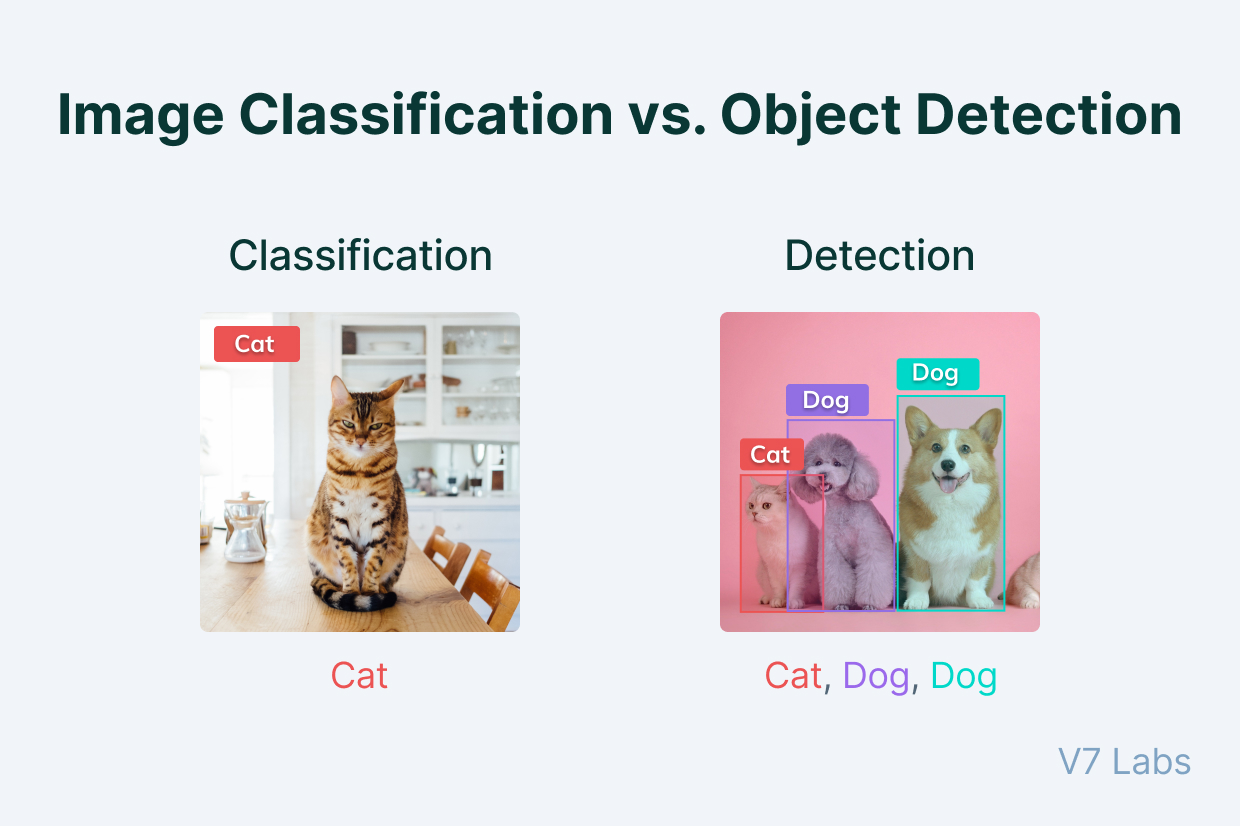
\includegraphics[scale=0.5]{gambar/object_detection_vs_image_recognition.jpg}
%     \caption{Ilustrasi Perbedaan Antara \textit{Object Detection} dan \textit{Image Recognition.}}
%     \label{fig:objectdetcompare}
% \end{figure}

\section{\textit{Convolutional Neural Network (CNN)}}
\label{sec:convolutionalneuralnetwork}
CNN merupakan algoritma \textit{deep learning} yang mampu mengambil masukan berupa gambar, menetapkan prioritas untuk berbagai aspek/objek dalam gambar dan mampu membedakan satu sama lain. Tahapan \textit{pre-processing} yang dibutuhkan CNN lebih sedikit jika dibandingkan dengan algoritma klasifikasi lainnya \citep*{towardsDS}. \textit{Convolutional Neural Network (CNN)} itu sendiri juga merupakan pengembangan dari \textit{Multilayer Percepton (MLP)} yang didesain untuk mengolah data dua dimensi. CNN termasuk dalam jenis \textit{Deep Neural Network} karena kedalaman jaringan yang tinggidan banyak diaplikasikan pada data citra \citep*{putra2016klasifikasi}.\par
Secara sederhana, CNN memiliki beberapa jenis \textit{neural layers} yang masing-masing memiliki peranannya masing-masing \citep*{voulodimos2018deep}. Adapun secara sederhana CNN terdiri dari 3 jenis utama \textit{neural layers} yaitu: \par
\begin{enumerate}[nolistsep]
    \item \textit{Convolutional Layer}
    \item \textit{Pooling Layer}
    \item \textit{Subsampling Layer}
    \item \textit{Fully Connected Layer}
\end{enumerate}
\par
Secara umum, cara kerja CNN hampir serupa pada MLP, hanya saja dalam CNN setiap neuron dipresentasikan dalam bentuk dua dimensi. Adapun cara kerja dari suatu MLP sederhana yaitu MLP semula memiliki sejumlah \textit{layer} dengan masing-masing layer memiliki sejumlah \textit{neuron}. MLP menerima masukan data dalam bentuk satu dimensi, kemudian mempropagasikan data tersebut pada jaringan sehingga didapat hasil keluaran. Setiap hubungan antar \textit{neuron} pada dua \textit{layer} yang bersebelahan memiliki parameter bobot satu dimensi yang menentukan kualitas mode. Disetiap data input pada layer dilakukan operasi linear dengan nilai bobot yang ada, kemudian hasil komputasi akan ditransformasi menggunakan operasi non linear yang disebut sebagai fungsi aktivasi. \par

\subsection{\textit{Region Based Convolutional Neural Network (R-CNN)}}
\label{subsec:regionbasedconvolutionalneuralnetwork}

\section{\textit{Evaluation Metrics}}
\label{sec:evaluationmetrics}

\subsection{\textit{Mean Average Precision (mAP)}}
\label{subsec:meanaverageprecision}

\subsection{\textit{Confusion Metrics}}
\label{subsec:confusionmetrics}

\subsection{F1 \textit{Scores}}
\label{subsec:f1scores}

\subsection{\textit{Intersect over Union (IoU)}}
\label{subsec:intersectoverunion}

% keknya gaperlu ??
% \section{Word Segmentation}
% \label{sec:wordsegmentation}
% Pengenalan tulisan tangan merupakan Teknik untuk menginterpretasikan tulisan tangan kedalam bentuk digital. Proses pengenalan tulisan tangan dapat diperoleh dengan 2 cara yaitu dengan mengonversi otomatis karakter pada saat ditulis pada layar sentuh dengan pena digital dan cara lain yaitu dengan melakukan pengambilan gambar serta pemrosesan gambar pada suatu teks yang ingin dikenali [8]. Pada proses segmentasi huruf, mulanya dokumen gambar disegmentasi kedalam baris-baris teks. Kemudian, algoritma segmentasi huruf diterapkan pada satu baris teks tersebut. Pada satu baris teks tersebut, secara umum proses segmentasi huruf konvensional menjalankan algoritma yang terdiri dari 2 tahapan yaitu: ekstraksi kandidat huruf berdasarkan pemisah huruf dan dilanjut dengan klasifikasi kandidat huruf \citep*{ryu2015word}.

\section{\textit{You Only Look Once (YOLO)}}
\label{sec:yolo}
YOLO merupakan salah satu arsitektur dari CNN yang dioptimasi untuk mendeteksi objek pada gambar. Arsitektur YOLO sangat cepat apabila dibandingkan dengan arsitektur pengenalan objek lainnya . YOLO melakukan proses pengenalan objek berbasis CNN dalam sebuah kotak yang disebut \textit{anchor} yang dipusatkan pada 13x13 \textit{grid cell} dalam sebuah gambar. Artinya, ukuran gambar diubah (dikurangi) menjadi 416x416 terlepas dari ukuran asli dari gambar yang ingin di proses \textit{train or detect}. Artinya, jika terdapat perbedaan besar dalam rasio gambar yang diproses \textit{train}, maka akan terjadi distorsi serius pada objek ketika dilakukan proses penyesuaian ukuran\citep*{jeong2018image}. \par

\subsection{YOLOv5}
\label{subsec:yolov5}
% //TODO: tabel comparison yolov5

\section{\textit{Feature Extraction}}
\label{sec:featureextraction}